\def\mySecNum{1.4}
\mySection{\mySecNum~Buying and short-selling financial assets}
%-------------- start slide -------------------------------%{{{ 1
\begin{frame}[fragile,t]
	\frametitle{Transaction costs and the bid-ask spread}
\begin{mydefinition}
	The price at which one can buy is called the \textcolor{magenta}{offer price} or \textcolor{magenta}{ask price},
	and the price at which one can sell is called the \textcolor{magenta}{bid price}. The difference
	between the ask price and the bid price is called the \textcolor{magenta}{bid-ask spread}.
\end{mydefinition}
\bigskip
\bigskip

\begin{center}
	Terminology is in the perspective\\ of market-maker
	\bigskip

	\renewcommand{\arraystretch}{1.2}
	\begin{tabular}{|c|c|c|}
		\hline
                 & Ask (offer) price & Bid price \\ \hline
   End users     & Buy               & Sell      \\
   Market makers & Sell              & Buy       \\ \hline
	\end{tabular}
\end{center}
\end{frame}
%-------------- end slide -------------------------------%}}}
%-------------- start slide -------------------------------%{{{ 1
\begin{frame}[fragile,t]
\begin{center}
	Transaction costs \bigskip\bigskip

\renewcommand{\arraystretch}{1.2}
	\begin{tabular}{c|c}
		\textcolor{magenta}{Commission} & \textcolor{cyan}{bid-ask spread} \\ \hline
    Brokers                         & Market-makers                    \\
    Electronic trading system       &                                  \\ \hline
    Fixed amount per transaction    & Based on per share               \\
    or percentage of purchase price &                                  \\
	\end{tabular}
\end{center}
\end{frame}
%-------------- end slide -------------------------------%}}}
%-------------- start slide -------------------------------%{{{ 1
\begin{frame}[fragile,t]
	\begin{myexample}
		 Buy and sell 100 shares of XYZ with
		 \begin{center}
		 	 bid = \$49.75, \quad  offer = \$50, \quad  commission = \$15.
		 \end{center}
		 What is the transaction cost?
	\end{myexample}
	\bigskip
	\pause

	\begin{mysol}
		\begin{enumerate}
			\item Buy:
				\begin{align*}
					(100 \times \$50) + \$15 = \$5,015.
				\end{align*}
			\item Sell:
				\begin{align*}
					(100 \times \$49.75) - \$15 = \$4,960.
				\end{align*}
			\item Transaction cost:
				\begin{align*}
					 \$5,015 - \$4,960 = \$55.
				\end{align*}
		\end{enumerate}
		(Note that We have payed twice the commission.)
		\myEnd
	\end{mysol}
\end{frame}
%-------------- end slide -------------------------------%}}}
%-------------- start slide -------------------------------%{{{ 1
\begin{frame}[fragile,t]
	\frametitle{Ways to buy or sell}
	\begin{center}
	\renewcommand{\arraystretch}{1.2}
		\begin{tabular}{c|c|c|}
					 & \textcolor{magenta}{Market order} & \textcolor{cyan}{Limited order} \\ \hline
			Pros & Filled immediately                & Might not be filled             \\
			Cons & Price could be better             & At a better price               \\
		\end{tabular}
	\end{center}
	\bigskip

	\begin{enumerate}
		\item \textcolor{magenta}{Market order}: an instruction to trade a specific quantity of the asset
			immediately, at the best price that is currently available.
			\bigskip

		\item \textcolor{cyan}{Limited order}: an instruction to trade a specific quantity of the asset
			at a specified price.
			\bigskip

		\item Others such as \textcolor{red}{stop-loss order}.
	\end{enumerate}
\end{frame}
%-------------- end slide -------------------------------%}}}
%-------------- start slide -------------------------------%{{{ 1
\begin{frame}[fragile,t]
	\frametitle{Long vs short positions}
\begin{center}
	\begin{center}
		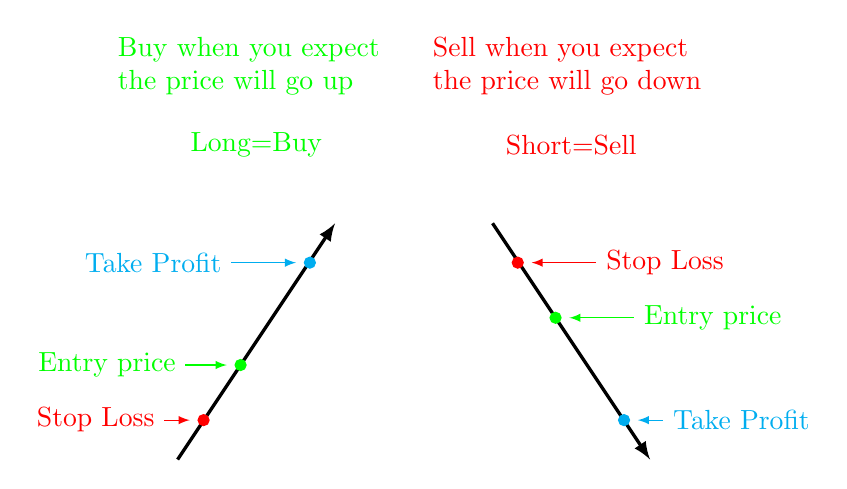
\begin{tikzpicture}[scale=1, transform shape]
			\tikzset{>=latex}
			% \node[green] (1) at (-2,3) {Lending};
			% \node[red] (1) at (2,3) {Borrowing};

			\node[green,text width=10em] (1) at (-2,2) {Buy when you expect the price will go up};
			\node[red,text width=10em] (1) at (2,2) {Sell when you expect the price will go down};
			\node[green] at (-2,1) {Long=Buy};
			\node[red] at (2,1) {Short=Sell};

			\draw[->,very thick] (-3,-3) -- (-1,0);
			\draw[->,very thick] (1,0) -- (3,-3);
			\filldraw[red] (-2.67,-2.5) circle (2pt);
			\draw [<-,red, shorten <= 0.5em] (-2.67,-2.5) -- ++ (-0.5,0) node [left] {Stop Loss};
			\filldraw[cyan] (2.67,-2.5) circle (2pt);
			\draw [<-,cyan, shorten <= 0.5em] (2.67,-2.5) -- ++ (0.5,0) node [right] {Take Profit};
			\filldraw[red] (1.32,-0.5) circle (2pt);
			\draw [<-,red, shorten <= 0.5em] (1.32,-0.5) -- ++ (1,0) node [right] {Stop Loss};
			\filldraw[cyan] (-1.32,-0.5) circle (2pt);
			\draw [<-,cyan, shorten <= 0.5em] (-1.32,-0.5) -- ++ (-1,0) node [left] {Take Profit};
			\filldraw[green] (-2.2,-1.8) circle (2pt);
			\draw [<-,green, shorten <= 0.5em] (-2.2,-1.8) -- ++ (-0.7,0) node [left] {Entry price};
			\filldraw[green] (1.8,-1.2) circle (2pt);
			\draw [<-,green, shorten <= 0.5em] (1.8,-1.2) -- ++ (1,0) node [right] {Entry price};
			% \node[bride,minimum size=1.5cm] (T) at (-1,0) {};
			% \node[groom,mirrored,minimum size=1.5cm] (N) at (1,0) {};
		\end{tikzpicture}
	\end{center}
\end{center}
\end{frame}
%-------------- end slide -------------------------------%}}}
%-------------- start slide -------------------------------%{{{ 1
\begin{frame}[fragile]
	\frametitle{Short-selling}
\begin{center}
	\begin{tikzpicture}[scale=1, transform shape]
		\tikzset{>=latex}
		\node[businessman,minimum size=3em] (T) at (-3,0) {Broker};
		\node[duck,mirrored,minimum size=3em] (N) at (0,0) {Short seller};
		\node[judge,mirrored,minimum size=3em] (N) at (3,0) {Market};
		\draw [->] (-2,0.5) -- (-1,0.5);
		\draw [->] (-1,-0.5) -- (-2,-0.5);
		\draw [->] (1,0.5) -- (2,0.5);
		\draw [->] (2,-0.5) -- (1,-0.5);
		\node[text width=8em,align=center] at (-1.5,1.4) {Borrow shares at low price};
		\node[text width=4em,align=center] at (-1.5,-1.7) {Return shares};

		\node[text width=8em,align=center] at (1.5,1.4) {Sold at current market price};
		\node[text width=8em,align=center] at (1.5,-2.2) {When market price fall, buy them at lower price};
	\end{tikzpicture}
\end{center}
\end{frame}
%-------------- end slide -------------------------------%}}}
%-------------- start slide -------------------------------%{{{ 1
\begin{frame}[fragile,t]
\begin{myexample}
	Short-sell IBM stock for 90 days. \\
	\bigskip
\begin{center}
	\renewcommand{\arraystretch}{1.2}
	\begin{tabular}{|c|c|c|c| c|}
		\hline
             & Day zero      & Dividend Ex-Day & Day $90$        & Profit          \\ \hline
   Action    & Borrow shares &                 & Return shares   &                 \\
   Security  & Shell shares  &                 & Purchase shares &                 \\
	 Cash flow & $+S_0$        & $-D$            & $-S_{90}$       & $ S_0-D-S_{90}$ \\ \hline
	\end{tabular}
\end{center}
\end{myexample}
\end{frame}
%-------------- end slide -------------------------------%}}}
%-------------- start slide -------------------------------%{{{ 1
\begin{frame}[fragile,t]
Three reasons to short-sell
\begin{enumerate}
	\item Speculation
	\item Financing
	\item Hedging
\end{enumerate}

\bigskip
\mySeparateLine
\bigskip

Credit risk in short-selling
\begin{itemize}
	\item The lender holding the money with an extra called \textcolor{magenta}{Haircut}.
\end{itemize}
\bigskip

Interest received from lender
\begin{itemize}
	\item Scarcity decreases the interest rate.
	\item \textcolor{magenta}{Repo rate} in bound markets.
	\item \textcolor{magenta}{Short rebate} in the stock market.
\end{itemize}
\end{frame}
%-------------- end slide -------------------------------%}}}
